Strange attractors can be characterized by a measure that describes how the distance between adjacent trajectories changes in time.
\begin{figure}
	\centering
	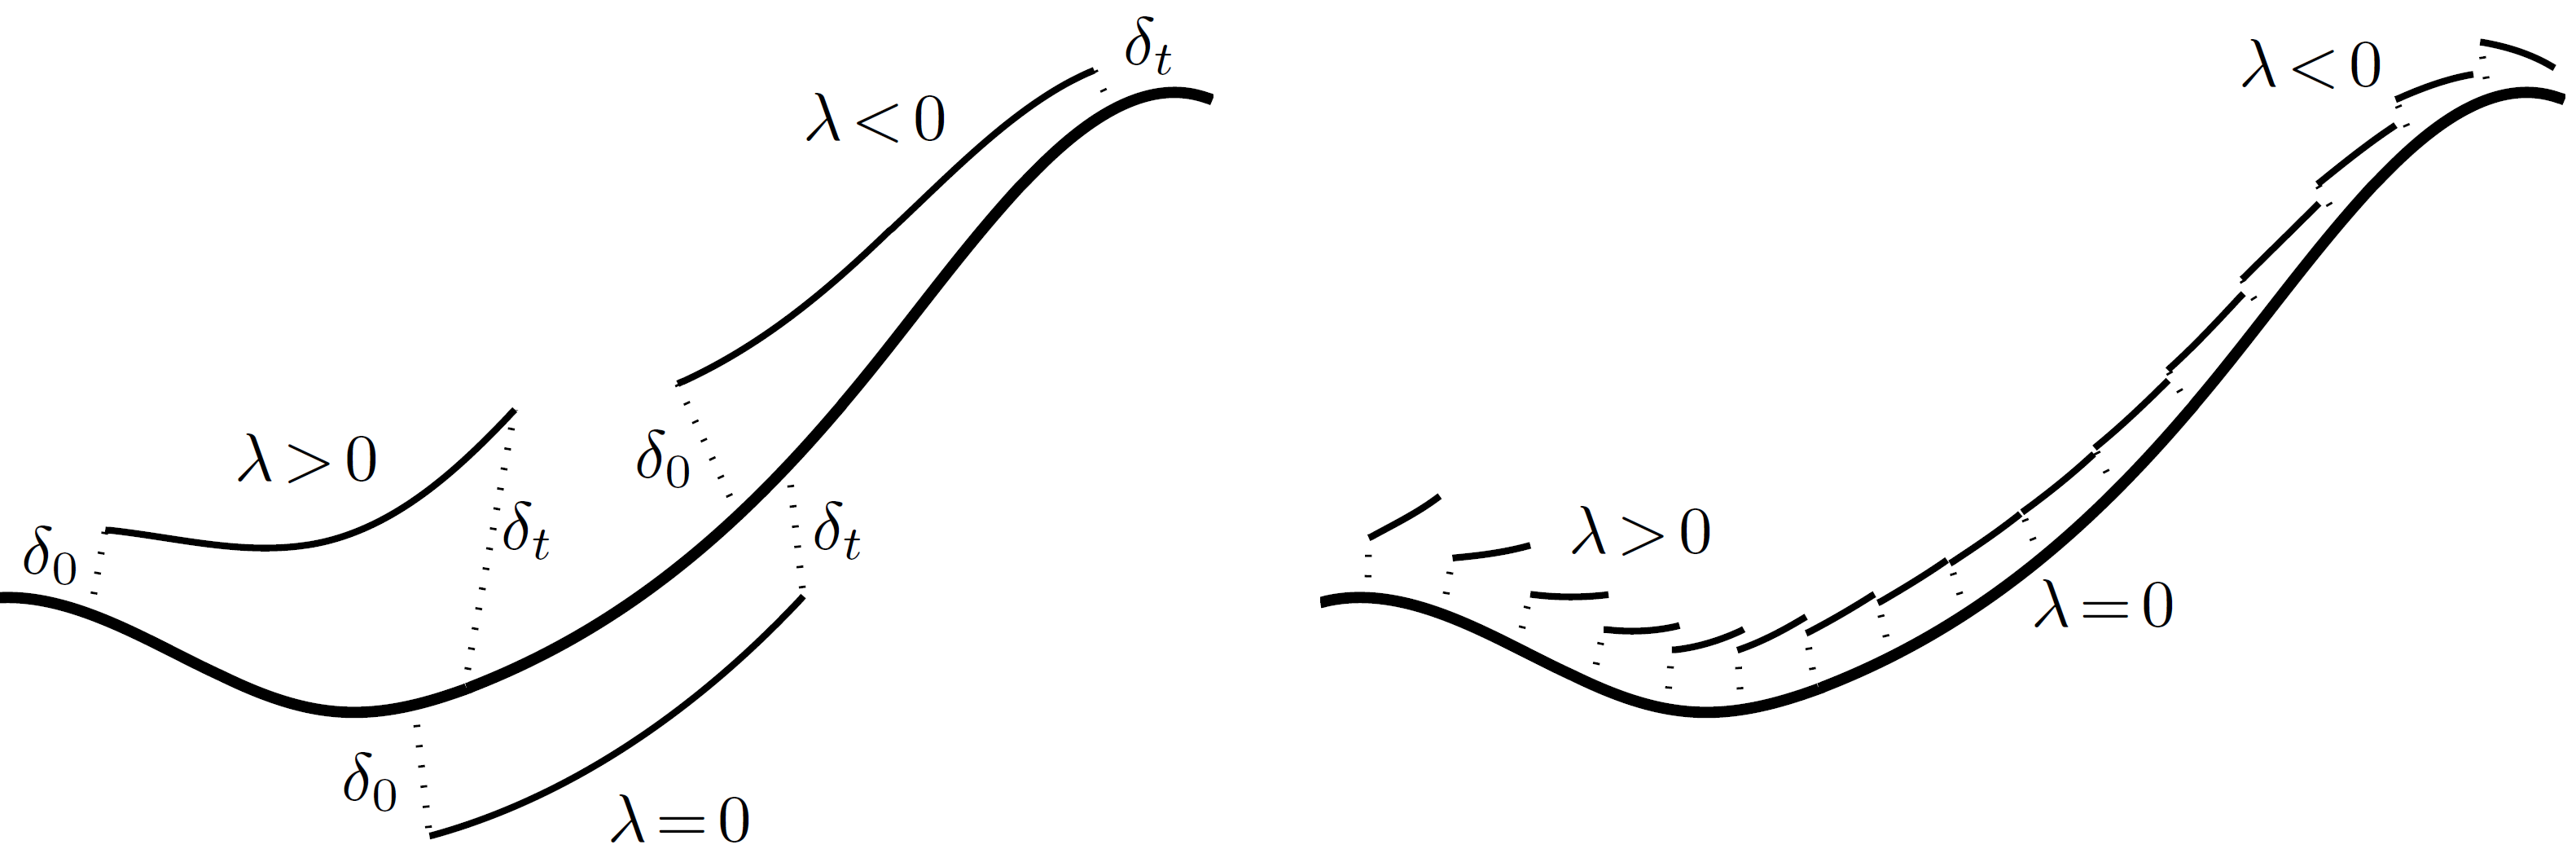
\includegraphics[width=0.7\linewidth]{lye.png}
	\caption{Left: Diverging, parallel and converging trajectories correspond to a local divergence rate of $\lambda>0, \lambda=0$ and $\lambda<0$, respectively.\\ Right: A Lyapunov exponent is determined as an average of the local divergence rate following close-by trajectories around the attractor.}
	\label{fig:lye}
\end{figure}
An example is shown in Figure (\ref{fig:lye} (left))  for the cases of diverging, parallel and converging trajectories.
For small initial distances $\delta_0$ and short times $t$ this behavior is determined by the local linearization. The distance between the two trajectories as a function of time is then given by
\begin{equation}
	\delta(t)=\delta_0e^{\lambda t}\quad\rightarrow\quad
	\lambda=\frac{1}{t}\ln\frac{\delta(t)}{\delta_0}
\end{equation}
where for $\lambda>0$ the trajectories are diverging, for $\lambda<0$ they are converging and for $\lambda=0$ the distance between corresponding points on the two trajectories does not change.
The exponent $\lambda$ is called the \emph{local divergence rate}, and as the name indicates, is a local quantity.\\
A global characterization is found by averaging the local divergence rate obtained from small segments of a trajectory over a long time by applying the procedure indicated in Figure (\ref{fig:lye} (right)).
In general, the sum over all Lyapunov exponents is negative for any attractor.
{\renewcommand{\arraystretch}{1.2}
\begin{table}[h!]
	\centering
	\caption{Classification of attractors in three dimensions.}
	\label{tab:catd}
	\begin{tabular}{c c c c}
		Type&$1^{st}$ exponent&$2^{nd}$ exponent&$3^{rd}$ exponent\\
		\hline
		Fixed Point&$-$ve&$-$ve&$-$ve\\
		Periodic orbit&0&$-$ve&$-$ve\\
		Quasi-Periodic orbit&0&0&$-$ve\\
		Strange attractor&$+$ve&0&$-$ve\\
		Lorenz attractor&0.906&0&$-$14.57\\
		R\"ossler attractor&0.0714&0&$-$5.39\\
	\end{tabular}
\end{table}}
\begin{theorem}[\textbf{Lyapunov Exponents}]
	If at least one of the average Lyapunov exponents is \emph{positive}, then the system is \textbf{chaotic}; if the average Lyapunov exponent is \emph{negative}, then the orbit is \textbf{periodic} and when the average Lyapunov exponent is \emph{zero}, a \textbf{bifurcation} occurs.
\end{theorem}